
\usetikzlibrary{positioning}
\tikzset{>=stealth}

\newcommand{\tikzmark}[3][]{\tikz[remember picture,baseline] \node [anchor=base,#1](#2) {$#3$};}

\section{Many-particle states, fermions}

\subsection{N-particle vacuum state}



Many-particle states will be built up by constructing a basis using products of single-particle states. 
Let $\lambda$ be some set of quantum numbers that uniquely specifies a single-particle quantum state.\\

\noindent Example: $\lambda$ could be the set of quantum numbers of the hydrogen-atom.\\
$\lambda = (n,l,m, \sigma)$\\
\begin{align*}
	n &: \text{Main quantum number.}\\
	l &: \text{Orbital angular momentum quantum number.}\\
	m &: \text{Quantization of angular momentum along z-axis.}\\ 
	\sigma &: \text{Spin quantum number.}
\end{align*}

\noindent Motion in 3 dimensions $\implies$ 3 quantum numbers : $(n,l,m)$\\
Spin: 1 quantum number.\\

\[ \begin{array}{ll}
\mbox{Corresponding state:} & \ket{n_\lambda}\\
\mbox{Adjoint state:} &  \bra{n_\lambda} = \left(\ket{n_\lambda} \right)^\dagger
\end{array}\] 



\noindent Vacuum-state (unoccupied state): $\ket{0_\lambda}$

\noindent Introduce creation and annihilation operators.

\[ \begin{array}{ll}
\mbox{Creation:} & \cd_\lambda\\
\mbox{Annihilation:} & c_\lambda
\end{array}\] 

\begin{align*}
	\ket{1_\lambda} &= \cd_\lambda \ket{0_\lambda}\\
	\ket{0_\lambda} &= c_\lambda \ket{1_\lambda}\\
	0 &= c_\lambda \ket{0_\lambda}
\end{align*}

\noindent In general, we will use a set og quantum numbers that are convenient. Exactly what this means in practice will become clear later, when we start looking at specific systems.\\

\noindent Many-body state:
\begin{align*}
	\ket{N}= \ket{ n_{\lambda_1}, n_{\lambda_2} ,n_{\lambda_3} ,...,  n_{\lambda_N}} 
\end{align*}

\noindent $\underline{\text{N-particle vacuum-state:}}$

\begin{align}
	&\ket{0} = \ket{0_{\lambda_1},0_{\lambda_2},...,0_{\lambda_N}}\\
	&\ket{N} : \text{Fock-basis} \nonumber
\end{align}

\noindent We regard fermions as quantized excitations of a matter field, in the same way as we regard photons as quantized excitations of an electromagnetic field.

Field operators for a fermion: $\psi^\dagger(x,t)$ : Creates a fermion in some quantum state at point $(\vec{r},s)=x$ at time t.
\begin{equation}
	\psi^\dagger(x,t)= \sum_\lambda \cd_\lambda(t) \varphi_\lambda^*(x)
\end{equation}

\noindent $\varphi_\lambda(\vec{r},s)$: Wave-function for quantum state with quantum numbers $\underline{\lambda}$.\\

\noindent Quantization:
\begin{equation}
	\{\psi^\dagger (x,t), \psi(x,t) \}= \delta(\vec{r}-\vec{r'}) \delta(s,s')
\end{equation}

Note that $t$ is the same in $\psi^\dagger$ and $\psi$!
\begin{equation}
	\{A,B\}= AB+BA
\end{equation}

\noindent The set of wavefunctions $\varphi_\lambda(\vec{r})$ are assumed to constitute a $\underline{\text{complete set}}$ i.e. any function $f(\vec{r})$ can be expressed in terms of $\{\varphi_\lambda(\vec{r})\}$

\begin{equation}
	f(\vec{r},s) = \sum_\lambda a_\lambda \varphi_\lambda (\vec{r}, s)
\end{equation}

$\{ \varphi_\lambda(\vec{r},s) \}$ is furthermore assumed to be orthonormalized

\begin{equation}
	\sum_{\vec{r},s} \varphi_\lambda^* (\vec{r},s) \varphi_{\lambda'} (\vec{r},s) = \delta_{\lambda, \lambda'},
\end{equation}

where 
\[
	\delta_{\lambda, \lambda'}=
\begin{cases}
	1;& \lambda = \lambda'\\
	0; & \lambda \neq \lambda' 
\end{cases}
\]

\begin{align*}
	\sum_{\vec{r}} \varphi_{\lambda'}^*(\vec{r},s) f(\vec{r},s) &= \sum_\lambda \sum_{\vec{r}} \varphi_{\lambda'}^*(\vec{r},s) \varphi_\lambda(\vec{r},s)\\
	&= \sum_\lambda \delta_{\lambda, \lambda'}\\
	&= \lambda'
\end{align*}

\begin{align*}
	f(\vec{r},s) &= \sum_\lambda \sum_{\vec{r'},s} \varphi_\lambda^* (\vec{r'},s') f(\vec{r},s') \varphi_\lambda (\vec{r},s)\\
	&= \sum_{\vec{r'},s'} \left[ \sum_\lambda \varphi_\lambda^* (\vec{r'},s') \varphi_\lambda (\vec{r},s) \right] f(\vec{r'},s') \\
	&= \sum_{\vec{r'},s'} \delta(\vec{r}-\vec{r'}) \delta_{s,s'} f(\vec{r'},s')
\end{align*}
 
\subsection{Completeness relation}

\begin{equation}
	\sum_\lambda \varphi_\lambda^* (\vec{r},s) \varphi_\lambda(\vec{r},s) = \delta(\vec{r}-\vec{r'}) \delta_{s,s'}
\end{equation}

Futhermore:

\begin{align}
	\{ \psi^\dagger(x',t), \psi(x,t) \} &= \delta_{x',x} \label{complete_1} \\
	&= \sum_{\lambda_1} \sum_{\lambda_2} \{\cd_{\lambda_1}, c_{\lambda_2} \} (\vec{r},s)  \varphi_{\lambda_1}^* (\vec{r},s) \varphi_{\lambda_2} \nonumber
\end{align}

If $\{\cd_{\lambda_1}, c_{\lambda_2}\}= \delta_{\lambda_1, \lambda_2}$ then equation \eqref{complete_1} is satisified.

\begin{equation}
	\{\cd_{\lambda_1}, c_{\lambda_2}\}= \delta_{\lambda_1, \lambda_2}
\end{equation}

\noindent $\underline{\text{In addition:}}$

\begin{align}
	\{ \psi^\dagger(x',t), \psi^\dagger(x,t) \} &= 0 \implies \{\cd_{\lambda'}, cd_\lambda\} =0\\
	\{ \psi(x',t), \psi(x,t) \} &= 0 \implies \{c_{\lambda'}, c_\lambda\} =0\\
	\cd_\lambda \cd_\lambda \ket{0}&=0
\end{align}
Cannot create more than one fermion in one single-particle state. (Pauli-principle) $\implies$

\begin{align*}
	c_\lambda c_\lambda \ket{n_\lambda}&=0\\
	\{\cd_{\lambda_1},c_{\lambda_2}\}&= \delta_{\lambda_1, \lambda_2}\\
	\lambda_1 \neq \lambda &:\\
	\ket{n_{\lambda_1} n_{\lambda_2}} &= - \ket{n_{\lambda_2} n_{\lambda_1}}
\end{align*}

\noindent A fermionic two-particle sstate is antisymmetric under interchange of the constituent single-particle states.

\begin{tcolorbox}
	The next step is now to express operators representing observables in terms of creation and destruction operators. This is called $\underline{\text{second quantization}}$.
\end{tcolorbox}

\subsection{Operators}

\noindent \uline{Definitions:}

\begin{enumerate}
	\item
		One-particle operator is an operator representing an observable of the following classical form
		\begin{equation}
			U= \sum_{i=1}^{N} U_i(\vec{r_i}, \vec{p_i}).
		\end{equation}
		$U_i$ depends only on the coordinate and momentum of one particle $(\vec{r_i}, \vec{p_i})$.
	\item
		Two-particle operator is an operator representing an observable of the following classical form
		\begin{equation}
			V= \sum_{i,j } V_{ij} (\vec{r_i}, \vec{p_i},\vec{r_j}, \vec{p_j}).
		\end{equation}
		$V_{ij}$ depends on the coordinates and momenta of two particles, $(\vec{r_i}, \vec{p_i})$ and $(\vec{r_j}, \vec{p_j})$. For the situations we will consider $V_{ij}$ will depend only on $\vec{r_i}$ and $\vec{r_j}$, not $\vec{p_i}, \vec{p_j}$.
\end{enumerate}

\noindent \uline{Matrix elements of single-particle operators.}



\begin{equation*}
	\hat{U} \ket{N}= \sum_i \hat{U_i} \ket{N}
\end{equation*}

$\hat{U_i}$ Only works on $\underline{one}$ element in $\ket{N}$:




	

\begin{equation*}
	\hat{U}_i = \tikzmark{node1}{\hat{U}_i}\ket{n_{\lambda_1},\cdots, \tikzmark[black]{node2}{n_{\lambda_i}}, \cdots, n_{\lambda_N}} 
\end{equation*}
\begin{tikzpicture}[overlay, remember picture,node distance =1.5cm]
	\draw[->,black] (node1) .. controls +(down:1.2cm) and +(right:0cm) .. node[below] {Works on this element \uline{only}} (node2.south);
\end{tikzpicture}
\linebreak


\noindent \uline{Examples of one-particle operators:}

\begin{enumerate}
	\item
		Kinetic energy $T$
		\begin{equation}
			\hat{T}= \sum_{i=1}^{N} \frac{\hat{p_i}^2}{2m} \ket{N},
		\end{equation}
		spin-independent (does not involve spin-coordinate).
	\item
		Crystal potential that electrons move through in a solid
		\begin{align}
			\hat{V} &= \sum_i \hat{V_i} \ket{N}\\
			\hat{V_i} &= \sum_j \hat{V}_{ij} (\vec{r_i}-\vec{R_j}),
		\end{align}
		spin-independent, (no spin-coordinate).\\
		$\vec{r_i}:$ Electron-coordinate\\
		$\vec{R_j}:$ Ion-coordinate
\end{enumerate}

\noindent The matrix element of a 1-p operator sandwiched between two many-particle states:

\begin{align}
	\bra{N'} \hat{U}\ket{N} &= \sum_i  \bra{N'} \hat{U_i}\ket{N} \nonumber \\
	&= \sum_i \bra{n'_1, \cdots, \tikzmark{node1}{n'_i}, \cdots, n'_N}\tikzmark{node2}{\hat{U_i}} \ket{n_1, \cdots, \tikzmark{node3}{n_i},\cdots, n_N} \nonumber
	\begin{tikzpicture}[overlay, remember picture,node distance =1.5cm]
		\draw[->,black] (node2) .. controls +(down:1.2cm) and +(right:0cm) .. node[below] {i-th element} (node3.south);
	\end{tikzpicture}\\
	\nonumber \\
	&= \sum_i \bra{\tilde{N'}}\ket{\tilde{N}} \bra{n'_i} U_i \ket{n_i}\\
	\ket{\tilde{N}} &= \prod_{k \neq i} \ket{n_k} \nonumber \\
	\ket{\tilde{N'}} &= \prod_{k \neq i} \ket{n'_k} \nonumber
\end{align}

\noindent \uline{Normalization:}

\begin{align}
	\frac{\bra{N'} \hat{U} \ket{N}}{\braket{N'}{N}} &= \sum_i \frac{\bra{\tilde{N'}} \ket{\tilde{N}}}{\braket{\tilde{N'}}{\tilde{N}}} \cdot \frac{\bra{n'_i} \hat{U_i} \ket{n_i}}{{\braket{n'_i}{n_i}}} \nonumber \\
	&= \sum_i \frac{\bra{n'_i} \hat{U_i} \ket{n_i}}{\braket{n'_i}{n_i}}
\end{align}


\begin{tcolorbox}
	One-particle operators are defined by matrix-elements in a one-particle Hilbert-space $\{\ket{n_i}\}$, ${i=1,\cdots,N}$.
\end{tcolorbox}

\noindent Matrix elements of \uline{two-particle operators}

\begin{equation}
	\hat{V} \ket{N}= \sum_{i,j} \tikzmark{node1}{\hat{V}_{ij}} \ket{n_1, \cdots , \tikzmark{node2}{n_i}, \cdots, \tikzmark{node3}{n_j}, \cdots, n_N}
	\begin{tikzpicture}[overlay, remember picture,node distance =1.5cm]
		\draw[->,black] (node1) .. controls +(down:1.2cm) and +(right:0cm) .. node[below] {} (node2.south);
		\draw[->,black] (node1) .. controls +(down:1.2cm) and +(right:0cm) .. node[below] {Works only on these two elements} (node3.south);
	\end{tikzpicture}\\
\end{equation}\\
\linebreak

\noindent \uline{Example: Coulomb-interactions}

\noindent Matrix element:

\begin{align}
	\bra{N'} \hat{V} \ket{N} &= \sum_{i,j} \bra{n'_1, \cdots , n'_i, \cdots, n'_j, \cdots, n'_N} \hat{V}_{ij} \ket{n_1, \cdots , n_i, \cdots, n_j, \cdots, n_N}\\
	&= \sum_{i,j} \prod_{k\neq (i,k)} \braket{n'_k}{n_k} \bra{n'_i, n'_j} \hat{V}_{ij} \ket{n_i, n_j}
\end{align}
\noindent \uline{Normalization:}

\begin{equation}
	\frac{\bra{N'} \hat{V} \ket{N}}{\braket{N'}{N}} = \sum_{ij} \frac{\bra{n'_i, n'_j}\hat{V_{ij}}\ket{n_i, n_j}}{\braket{n'_i,n'_j}{n_i,n_j}}
\end{equation}

\begin{tcolorbox}
	Matrix elements of two-particle operators are computed in a Hilbert-space of two-particle states.
\end{tcolorbox}

\noindent For the 2-particle operators we consider

\begin{align}
	\hat{V}_{ij} &= \hat{V}_{ji}, \hspace{1cm} i \neq j\\
	\text{If } i=j \implies \hat{V}_{ij} &=0, \nonumber 
\end{align}
because otherwise a 2-particle operator would operate on a 1-particle state, which it does not.\\
\linebreak

\noindent \uline{Interacting electron gas in a periodic crystal potential $U(\vec{r})$}


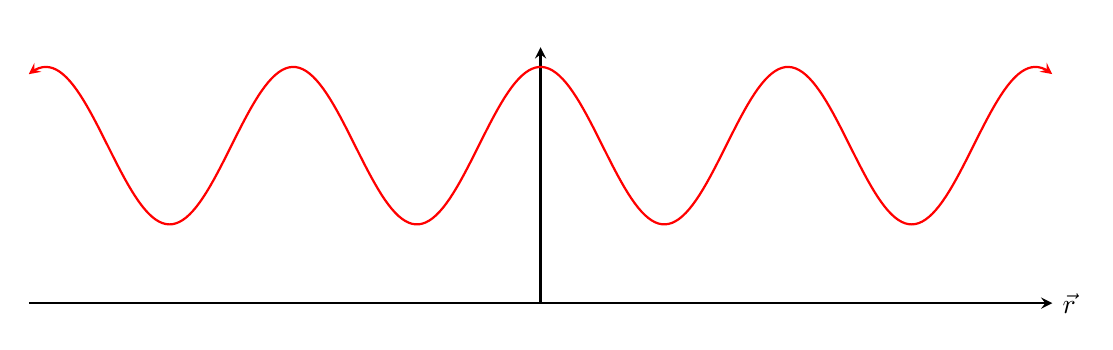
\begin{tikzpicture}[
	tl/.style = {% tick labels
		fill=white, inner sep=1pt, font=\scriptsize,},
	]
	
	% axes
	\draw[->,thick] (-6.5,-2) -- (6.5,-2) node[right] {$\vec{r}$};
	\draw[->,thick] (0,-2) -- (0, 1.25) node[above] {$$};
	% curve
	\draw[<->,thick,draw=red,
	domain=-6.5:6.5,samples=300,variable=\x] 
	plot (\x,{cos(deg{\x*2})});

\end{tikzpicture}

\begin{equation}
	H = \sum_i \left[\frac{\vec{p_i}^2}{2m} + U(\vec{r_i})  \right]+ \sum_{ij} V_{e-e}^C (\vec{r_i}-\vec{r_j})
\end{equation}

\noindent This is, in general, a very hard problem to solve. In particular, it is the Coulomb-term which makes it really hard.\\
\linebreak

\noindent\uline{One-particle term:}
\begin{align}
	&H_1 = \sum_i H_1 (\vec{r_i}, \vec{p_i})\\
	&H_1 (\vec{r_i}, \vec{p_i}) = \frac{\vec{p_i}^2}{2m} + U(\vec{r_i})
\end{align}
\linebreak
\noindent \uline{Two-particle term:}
\begin{equation}
	H_2 = \sum_{ij} V_{e-e}^C (\vec{r_i}-\vec{r_j}
\end{equation}

\noindent We will first work out the second-quantized form of the two terms in $H_1 (\vec{r_i}, \vec{p_i})$. \\
\linebreak

\noindent We define $\varphi_\lambda ( \vec{r},s)$ as follows:
Solutions to the single-particle Schrödinger-equation

\begin{align}
	&H_1 \varphi_\lambda = \varepsilon_\lambda \varphi_\lambda\\
	&H_1 = -\frac{\hbar^2}{2m} \vec{\laplacian} + U(\vec{r}) ; \hspace{0.5cm} \vec{\laplacian} : \text{Laplace-operator} \label{h_1}
\end{align}

\noindent The task is now to find a second-quantized form of $H_1$ which will yield the \uline{same} matrix elements as \ref{h_1}.\\
\linebreak
\noindent Consider:
\begin{equation}
	\bra{\lambda_1} H_1 \ket{\lambda_2} ; \hspace{0.5cm} \braket{\lambda_1}{\lambda_2} = \delta_{\lambda_1, \lambda_2}
\end{equation}

\noindent \uline{Completeness relation:}

\begin{align}
	&\braket{\vec{r},s}{\lambda_1} = \varphi_{\lambda_{1}} \hspace{0.5cm} \text{(some wavefunction)} \nonumber\\
	&\text{Normalized states: } \braket{\lambda}{\lambda}=1 \nonumber \\
	&\sum_\lambda \varphi_\lambda^* (\vec{r},s) \varphi_\lambda (\vec{r'},s') = \delta(\vec{r}-\vec{r'}) \delta_{s,s'}\\
	&\sum_{\vec{r},s} \varphi_{\lambda'}^* (\vec{r},s) \varphi_\lambda (\vec{r},s) = \delta_{\lambda, \lambda'}\\
	& \braket{\lambda}{\lambda'}= \delta_{\lambda, \lambda'} \implies \sum_{\vec{r},s} \ket{\vec{r},s} \bra{\vec{r},s} = 1 ; \hspace{0.3cm} \sum_x \ket{x}\bra{x}=1
\end{align}

\noindent Now we use this version of the completeness relations to evaluate the matrix element $\bra{\lambda_1} H_1 \ket{\lambda_2}$

\begin{align}
	\bra{\lambda_1} H_1 \ket{\lambda_2} &= \sum_{\vec{r},s} \sum_{\vec{r'},s'} \braket{\lambda_1}{\vec{r},s} \bra{\vec{r},s} H_1 \ket*{\vec{r'},s'} \braket*{\vec{r'}}{\lambda_2}\\
	&=  \sum_{\vec{r},s} \sum_{\vec{r'},s'} \varphi_{\lambda_1}^* (\vec{r},s)  \bra{\vec{r},s} H_1 \ket*{\vec{r'},s'} \varphi_{\lambda_2} (\vec{r'},s') \nonumber
\end{align}

\begin{align}
	&H_1 = \frac{\vec{p}^2}{2m}+ U(\vec{r}) \hspace{1cm} \text{Classical}\\
	&\vec{p}= \frac{\hbar}{i} \vec{\gradient}  ;  \hspace{1cm} \vec{\gradient}: \text{Gradient operator}\\
	&H_1 =  - \frac{\hbar^2 \vec{\laplacian}}{2m} + U(\hat{r}) \hspace{1cm} \text{Quantum mechanical}\\
	& U(\hat{r}) \ket{r} = U(\vec{r})\ket{r}
\end{align}

\noindent $\vec{r}:$ Position : eigenvalue of the position operator

\begin{align}
	\hat{r} \ket{\vec{r},s}= \vec{r} \ket{\vec{r}, s}\\
	U(\hat{r}) \ket{\vec{r},s}= U(\vec{r}) \ket{\vec{r},s}
\end{align}


\begin{align}
	\bra{\vec{r},s} H_1 \ket*{\vec{r'},s'} &= \left[-\frac{\hbar^2}{2m} \vec{\laplacian}+ U(\vec{r}) \right] \delta_{\vec{r}, \vec{r'}} \delta_{s,s'}\\
	\bra{\lambda_1} H_1 \ket{\lambda_2} &= \sum_{\vec{r},s} \varphi_{\lambda_1}^* (\vec{r},s) \left[-\frac{\hbar^2}{2m} \vec{\laplacian}+ U(\vec{r}) \right] \varphi_{\lambda_2} (\vec{r},s)\\
	&\equiv \varepsilon_{\lambda_1, \lambda_2} \nonumber
\end{align}

\noindent $\varphi_\lambda (\vec{r},s): $ Some complete set of functions, by assumption.\\
\linebreak
\noindent Let us now give an alternative form of $H_1$, which will yield the \uline{same} matrix elements.
\linebreak
\noindent \uline{Anzats:}

\begin{equation}
	H_1 = \sum_{\lambda_1, \lambda_2} h_{\lambda_1, \lambda_2} \cd_{\lambda_1} c_{\lambda_2}
\end{equation}
where $ h_{\lambda_1, \lambda_2}$ is some complex number.
Then:
\begin{align}
	\bra{\lambda_1} H_1 \ket{\lambda_2} &= \bra{0}c_{\lambda_1} \left(\sum_{\lambda'_1, \lambda'_2} h_{\lambda'_1, \lambda'_2} \cd_{\lambda'_1} c_{\lambda'_2} \right) \cd_{\lambda_2} \ket{0} \\
	&=\sum_{\lambda'_1, \lambda'_2} h_{\lambda'_1, \lambda'_2}  \bra{0}c_{\lambda_1}  \cd_{\lambda'_1} c_{\lambda'_2} \cd_{\lambda_2} \ket{0} \nonumber \\
	&= \sum_{\lambda'_1, \lambda'_2} h_{\lambda'_1, \lambda'_2}  \bra{0} (\delta_{\lambda_1, \lambda'_1}-\cd_{\lambda'_1}c_{\lambda_1} ) (\delta_{\lambda_2, \lambda'_2} -\cd_{\lambda_2} c_{\lambda'_2}) \ket{0} \nonumber\\
	&= \sum_{\lambda'_1, \lambda'_2} h_{\lambda'_1, \lambda'_2}  \delta_{\lambda_1, \lambda'_1} \delta_{\lambda_2, \lambda'_2} \braket{0}{0}\nonumber \hspace{1cm} (c_\lambda \ket{0} =0)  \\
	&= h_{\lambda_1, \lambda_2} \nonumber
\end{align}
Choose $ h_{\lambda_1, \lambda_2} = \varepsilon_{\lambda_1, \lambda_2}$ $\implies$ Same matrix-elements for
\begin{equation}
	H_1 = -\frac{\hbar^2}{2m} \vec{\laplacian}+ U(\hat{r}) 
\end{equation}
and
\begin{tcolorbox}
	\begin{equation}
		H_1 = \sum_{\lambda_1, \lambda_2} \varepsilon_{\lambda_1, \lambda_2} \cd_{\lambda_1} c_{\lambda_2} \label{sec_quant_h}
	\end{equation}
\end{tcolorbox}
Thus, \ref{sec_quant_h} is a useful 2nd quantized form of $H_1$.\\
\linebreak
\noindent This expression may be simplified. Consider now a judicial choice of the complete set $\{\varphi_\lambda(x) \}$:\\
\noindent Let ${\varphi_\lambda}$ be defined by

\begin{equation}
	\left(-\frac{\hbar^2}{2m} \vec{\laplacian}+ U(\vec{r})  \right) \varphi_\lambda(x) = \varepsilon_\lambda \varphi_\lambda(x)
\end{equation}
i.e. ${\varphi_\lambda}$ are eigenfunctions of $H_1$\\
\linebreak
\noindent Then:
\begin{align}
	\varepsilon_{\lambda_1, \lambda_2} &= \sum_x \varphi_{\lambda_1}^*(x)  \left(-\frac{\hbar^2}{2m} \vec{\laplacian}+ U(\vec{r})  \right) \varphi_{\lambda_2} (x)\\
	&=  \sum_x \varphi_{\lambda_1}^*(x) \varepsilon_{\lambda_2} \varphi_{\lambda_2}(x) \nonumber \\
	&= \varepsilon_{\lambda_2} \sum_x \varphi_{\lambda_1}^*(x) \varphi_{\lambda_2}(x)\nonumber \\
	&= \varepsilon_{\lambda_2} \delta_{\lambda_1, \lambda_2} \nonumber
\end{align}
giving that, 
\begin{equation}
	H_1 = \sum_{\lambda_1} \varepsilon_{\lambda_1} \cd_{\lambda_1} c_{\lambda_1}
\end{equation}

\noindent This form of $H_1$ has an intuitively appealing form: $  \cd_{\lambda_1} c_{\lambda_1}$ is a number operator. It counts the number of particles in state $\ket{\lambda_1}$.\\
\noindent $\varepsilon_\lambda$ is the single-particle energy in this state. Thus, $H_1$ is an operator that counts the energy in the system coming from all the possible states of the system.\\
\linebreak
\noindent General one-particle operators:
\begin{equation}
	T(x, \vec{p}) = T(x, \frac{\hbar}{i} \vec{\gradient}) 
\end{equation}
Could in principle depend on spin-coordinate $s$ !
\begin{equation}
	\bra{\lambda_1} T \ket{\lambda_2} = \sum_x \varphi_{\lambda_1}^*(x) T(x, \frac{\hbar}{i} \vec{\gradient}) \varphi_{\lambda_2}(x)
\end{equation}

\begin{tcolorbox}
	\begin{align}
		T &= \sum_{\lambda_1,\lambda_2} \bra{\lambda_1} T(x, \vec{p}) \ket{\lambda_2} \cd_{\lambda_1} c_{\lambda_2}\\
		&=\sum_{\lambda_1,\lambda_2} t_{\lambda_1,\lambda_2} \cd_{\lambda_1} c_{\lambda_2} \nonumber
	\end{align}
\end{tcolorbox}
\noindent This expression for $H_1$ and $T$ in second quantized form applies for any choice of sets of quantum numbers $\lambda$.\\
\linebreak
\noindent We next proceed by setting up a general form of second quantized form of 2-particle operators.





